\documentclass[conference]{IEEEtran}
\IEEEoverridecommandlockouts
% The preceding line is only needed to identify funding in the first footnote. If that is unneeded, please comment it out.
\usepackage{cite}
\usepackage{amsmath,amssymb,amsfonts}
\usepackage{algorithmic}
\usepackage{graphicx}
\usepackage{textcomp}
\usepackage{xcolor}
\def\BibTeX{{\rm B\kern-.05em{\sc i\kern-.025em b}\kern-.08em
    T\kern-.1667em\lower.7ex\hbox{E}\kern-.125emX}}
\begin{document}

\title{DRAFT: Reverse Image Search Documentation\\{\footnotesize May 1, 2022}}

\author{\IEEEauthorblockN{Jen McIntosh}
\IEEEauthorblockA{\textit{Brooklyn, NY \\
jgm9366@nyu.edu}}
\and
\IEEEauthorblockN{Shlok Goswami}
\IEEEauthorblockA{\textit{Brooklyn, NY \\
sg6862@nyu.edu}}
\and
\IEEEauthorblockN{
Ian Gray}
\IEEEauthorblockA{\textit{Brooklyn, NY \\
iwg210@nyu.edu}}
}

\maketitle

\begin{abstract}
ABSTRACT HERE!
\end{abstract}

\begin{IEEEkeywords}
CNN, sklearn, KNN, classifier, image search
\end{IEEEkeywords}

\section{Introduction}
\textit{"Describe the problem you are working on, why it’s important, and an overview of your results"} \\

The purpose of this project is to implement a system that can find faces with they are visible within queried images and videos, which later has applications in reverse-image searching. The system will search within a given dataset for a specific person of interest (POI) within the queried image. This sort of search is similar to pair matching or face verification.

\section{Related Work}
\textit{"Discuss published work that relates to your project. How is your approach similar or different from others?"}

\section{Dataset}
The pre-trained model implemented in ResNet50 is trained on imagenet, and we begin our reverse-image search by first passing the Labeled Faces in the Wild (LFW) dataset through the search. The results of the search will images from the LFW dataset which are most similar to the novel input image.

The ImageNet dataset consists of millions of pictures using a WorldNet hierarchy for data labels. It does not consist of solely human faces, as the LFW dataset does. Notably, roughly one fifth images within the ImageNet dataset include multiple objects, which has been shown by MIT researchers to lead to a 10\% drop in model accuracy\textsuperscript{1}. This setback will be discussed in later sections of this paper.

The LFW data set contains more than 13,000 images of faces, labeled with the name of the person pictured\textsuperscript{2}. The data set consists of several images which depict the same person. This is useful for the purposes of evaluating this reverse image search on faces, as inputting a face with known duplicates should result in a collection of similar images which contain multiple images of the same person.

\section{Methods}
\textit{"Discuss your approach for solving the problems that you set up in the introduction. Why is your approach the right thing to do? Did you consider alternative approaches? You should demonstrate that you have applied ideas and skills built up during the quarter to tackling your problem of choice. It may be helpful to include figures, diagrams, or tables to describe your method or compare it with other methods."}

\subsection{Baseline}
To establish our baseline reverse-image search we implemented a pre-trained deep learning ResNet50 model with its top layer removed, and then implemented a nearest neighbor algorithm. The RestNet50 model is pre-trained on imagenet, which is detailed in section III of this paper. The ResNet50 model converts images into just 2048 features, far fewer than other deep learning modules, which will expedite our search and nearest neighbor algorithm. Additionally, as the purpose of this model is to merely establish a baseline, the small number of features presents a potential area for (accuracy) improvement. We remove the top layer of ResNet50 so that the model returns convolved features rather than classification probabilities. We then fit our resulting feature vectors (consisting of 2048 features each) to one of sklearn's nearest neighbor algorithms. For the purposes of establishing a baseline we chose the ball\_tree algorithm. 

To implement a reverse-image search on faces, we first pass the lfw dataset through the RestNet50 pre-trained model and fit the resulting feature vectors to the nearest neighbor algorithm as previously described.From there we take the image to be "reverse searched," which is an image not present in the training dataset (hopefully), and again create the 2048 feature vector using ResNet50 and find its nearest neighbors from the lfw dataset. With the nearest neighbors' indices we are able to then return the most similar images from the lfw dataset.

\subsubsection{ResNet50 Architecture}

ResNet is short for Residual Networks, and it was one of the first neural networks to allow training of 150+ layered deep neural networks without the problem of vanishing gradients. Vanishing gradients often arise as network depth increases - as a gradient is back-propagated over several layers the repeated multiplication makes the gradient negligible. This phenomenon causes saturated, and eventually degrading, performance of the neural network. 

ResNet tackles the problem of vanishing gradients through the use of skip connections. Equation 2 summarizes, in essence, what a skip connection entails. The skip connection adds the original input layer to the convolved layer post-convolution, therefore the layers (original and convolved) must be of the same size. This is achieved by either outputting a convolved layer which is of the same size as the input, or by passing the original layer through a separate convolution layer resulting in the same size as the target convolved layer. Skip connections are applied prior to ReLU activation. kip connections are useful when dealing with vanishing gradients because they provide an alternate route for gradients AND they allow the model to learn an identity function. The identity function ensures that higher layers will not perform worse than lower layers.

The whole ResNet50 model consists of 5 stages, each with its own convolution and identity block. Each block has 3 convolution layers. Overall, the model has 23 million trainable parameters. The below figure illustrates the overall ResNet50 architecture along with the contents of the convolution and identity blocks.

\begin{figure}[h]
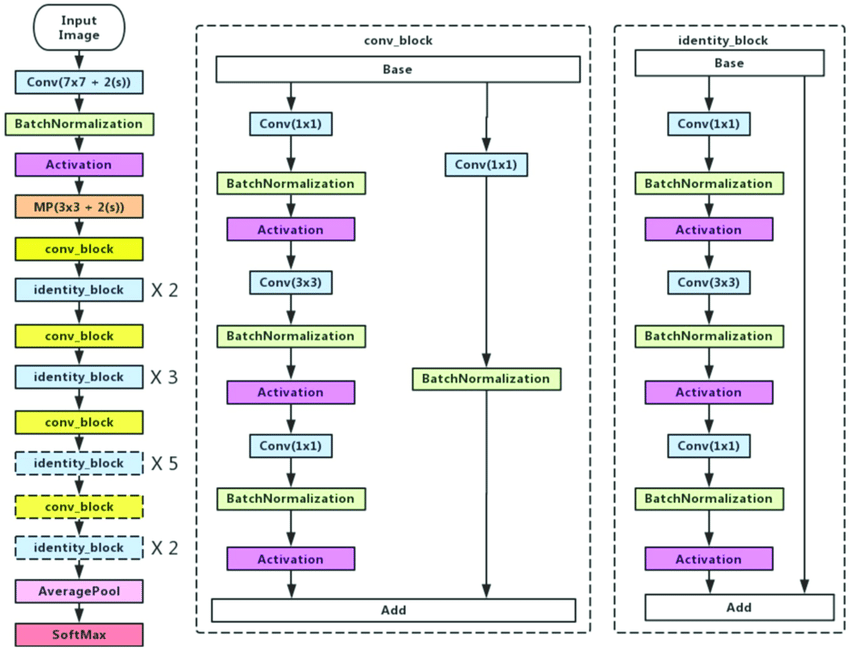
\includegraphics[width=7cm]{resnet50 arch.png}
\centering 
\caption{ResNet50 Architecture\textsuperscript{3}}
\label{fig:1}
\end{figure}

Note that in our model we do not include the final average pooling and soft max layers. These layers create an output of class probabilities, whereas without them the ResNet50 model outputs feature maps.

\subsubsection{$K$ Nearest Neighbors}
The $K$ Nearest Neighbors algorithm simply takes a new/input vector and finds the $k$ vectors within a stored train set which are "nearest" or "closest" to the input vector. It assigns the most frequent label amongst the $k$ neighbors to the new/input vector. Our KNN algorithm uses Euclidean distance as the metric to measure neighbor distance. Euclidean distance is defined as:

\begin{equation}
d_{ED}= \sqrt{ (x_1-y_1)^2 + (x_2-y_2)^2 + (x_3-y_3)^2 } \label{eq:1}
\end{equation}
Where $\textbf{x}=<x_1,x_2,x_3>$ and $\textbf{y}=<y_1,y_2,y_3>$ are vectors. This is also often called the L2 norm of $\textbf{x}-\textbf{y}$.

We first fit the results of the KNN algorithm run in the LFW dataset to the feature map produced by our model (2048 features), and use this to compare the new/input vector to the LFW dataset. Because of the large number of features, the KNN algorithm may be unable to accurately cluster similar features, and may be subject to overfitting, therefore we then reduced the size of our feature map to 1500 and used this to fit the KNN algorithm. 

\subsubsection{Baseline Results}
The below screenshots depict our input image and corresponding outputs, both before and after reducing the size of our feature map for KNN fitting. 

\begin{figure}[h]
    \centering
    \caption{Input Image for Establishing Baseline}
    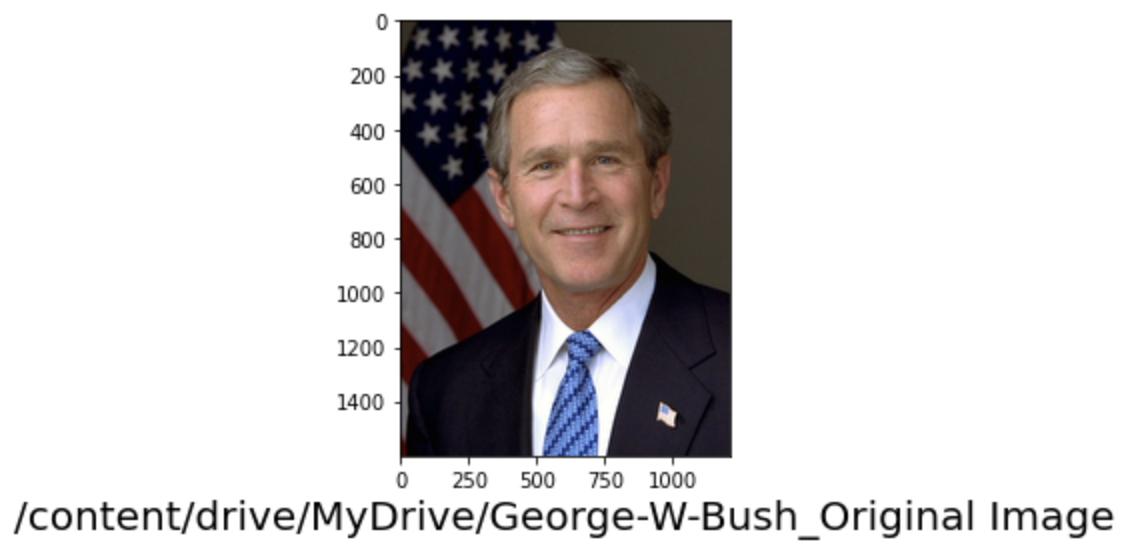
\includegraphics[width=7cm]{gwbush.png}
    \label{fig:2}

    \caption{Baseline Output Before Reducing FM Size}
    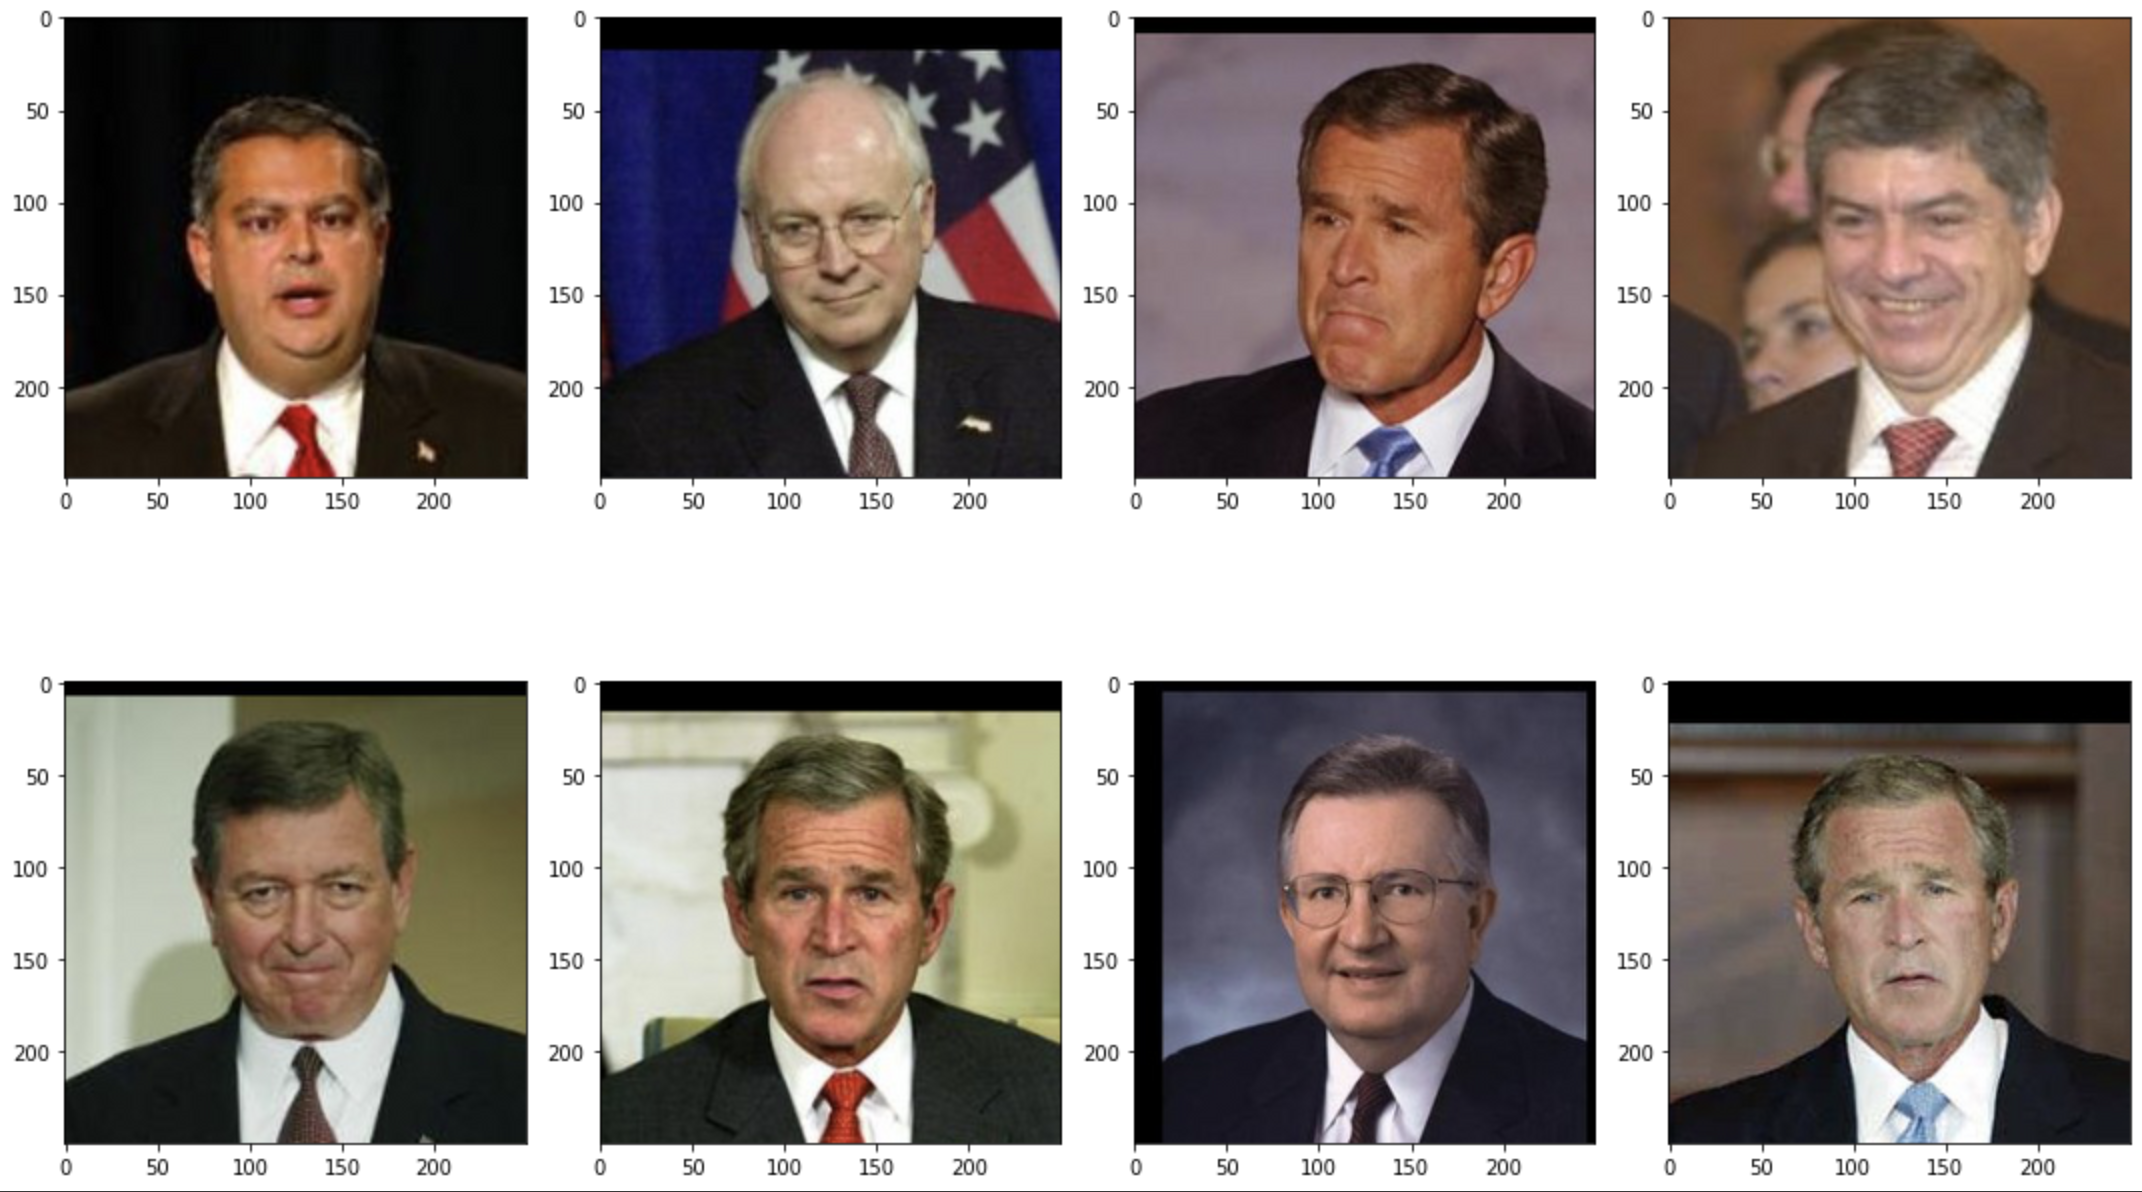
\includegraphics[width=7cm]{og_baseline.png}
    \label{fig:3}
    
    \caption{Baseline Output After Reducing FM Size}
    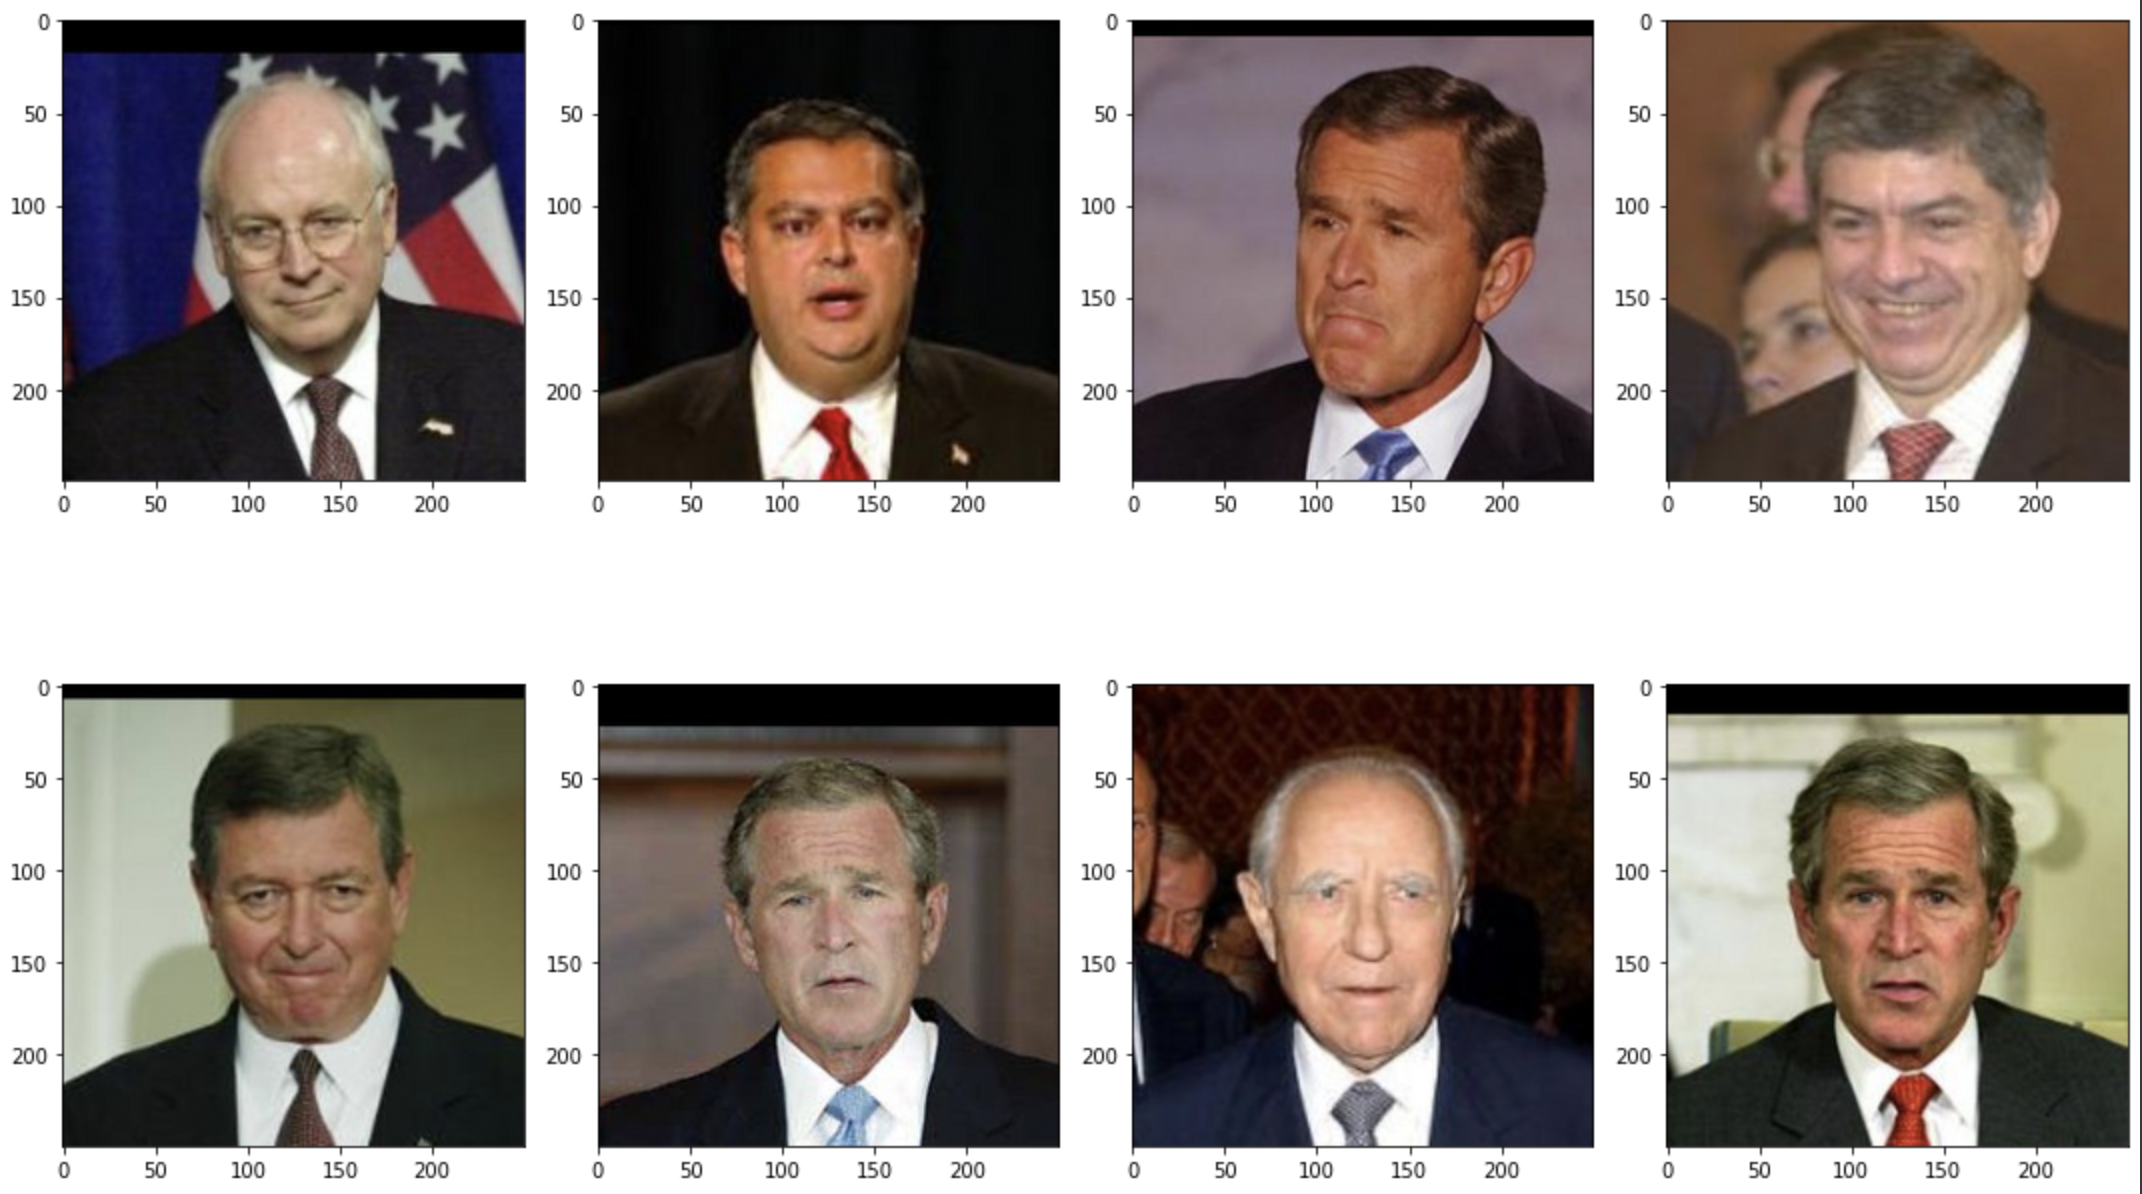
\includegraphics[width=7cm]{pca_baseline.png}
    \label{fig:4}
    \centering
\end{figure}

Interestingly enough, we noted that there was no noticeable improvement after reducing the size of our feature map, and with too many reductions ($<1000$ features) there was a degradation in search performance. This is something we address when we make improvements to this baseline.

\subsection{Improvements}
\textit{Here discuss how improvements were made upon baseline}\\

\textit{"Discuss the experiments that you performed to demonstrate that your approach solves the problem. The exact experiments will vary depending on the project, but you might compare with previously published methods, perform an ablation study to determine the impact of various components of your system, experiment with different hyperparameters or architectural choices, use visualization techniques to gain insight into how your model works, discuss common failure modes of your model, etc. You should include graphs, tables, or other figures to illustrate your experimental results."}



\section{Equations}
Here will be some relevant math if it ends up being necessary.....

\begin{equation}
   X_o+X_c = Add[X_o,X_c] :
   \label{eq:2}
\end{equation}
$$
\begin{bmatrix}
x_{1,1}^o & ... & x_{n,1}^o\\
... & ... & ...\\
x_{1,n}^o & ... & x_{n,n}^o\\
\end{bmatrix}
+
\begin{bmatrix}
x_{1,1}^c & ... & x_{n,1}^c\\
... & ... & ...\\
x_{1,n}^c & ... & x_{n,n}^c\\
\end{bmatrix}
$$
$$
=
\begin{bmatrix}
x_{1,1}^o+x_{1,1}^c & ... & x_{n,1}^o+x_{n,1}^c\\
... & ... & ...\\
x_{1,n}^o+x_{1,n}^c & ... & x_{n,n}^o+x_{n,n}^c\\
\end{bmatrix}
$$





\section{Conclusion}

\textit{"Summarize your key results - what have you learned? Suggest ideas for future extensions or new applications of your ideas."}\\

Some drawbacks to this model stemming from the LFW dataset:
\begin{itemize}
    \item Many groups are underrepresented by the LFW dataset, including babies, children, elderly people, and women.
    \item There are few instances of additional conditions such as low light, strong occlusion, and low resolution in the dataset.
    \item It is very difficult to extrapolate to N sized inputs.
    \item The dataset is not robust enough to create strong statistical conclusions about subgroups, and many minority ethnicities are either underrepresented or absent.
\end{itemize}

\begin{thebibliography}{00}
\bibitem{b1} https://venturebeat.com/2020/07/15/mit-researchers-find-systematic-shortcomings-in-imagenet-data-set/:text=MIT\%20researchers\% 20have\%20concluded\%20that,as\%20a\%20benchmark\%20data\%20set.
\bibitem{b2} http://vis-www.cs.umass.edu/lfw/index.html
\bibitem{b3} Ji, Qingge \& Huang, Jie \& He, Wenjie \& Sun, Yankui. (2019). Optimized Deep Convolutional Neural Networks for Identification of Macular Diseases from Optical Coherence Tomography Images. Algorithms. 12. 51. 10.3390/a12030051. 
\bibitem{b4} the quick brown fox
\bibitem{b5} jumps over
\bibitem{b6} the lazy dog
\bibitem{b7} nice
\end{thebibliography}
\vspace{12pt}
\color{red}
WOOOOO

\end{document}
